\begin{frame}{Small-Scale Features}
    \begin{block}{Causes}
        \begin{itemize}
            \item Retreat of glacier
            \item Sublimation
            \item Fracture
            \item Exposure of underlying rock
        \end{itemize}
    \end{block}
\end{frame}

\begin{frame}{Small-Scale Features}
\begin{figure}
\centering
\begin{subfigure}{0.48\textwidth}
    \centering
    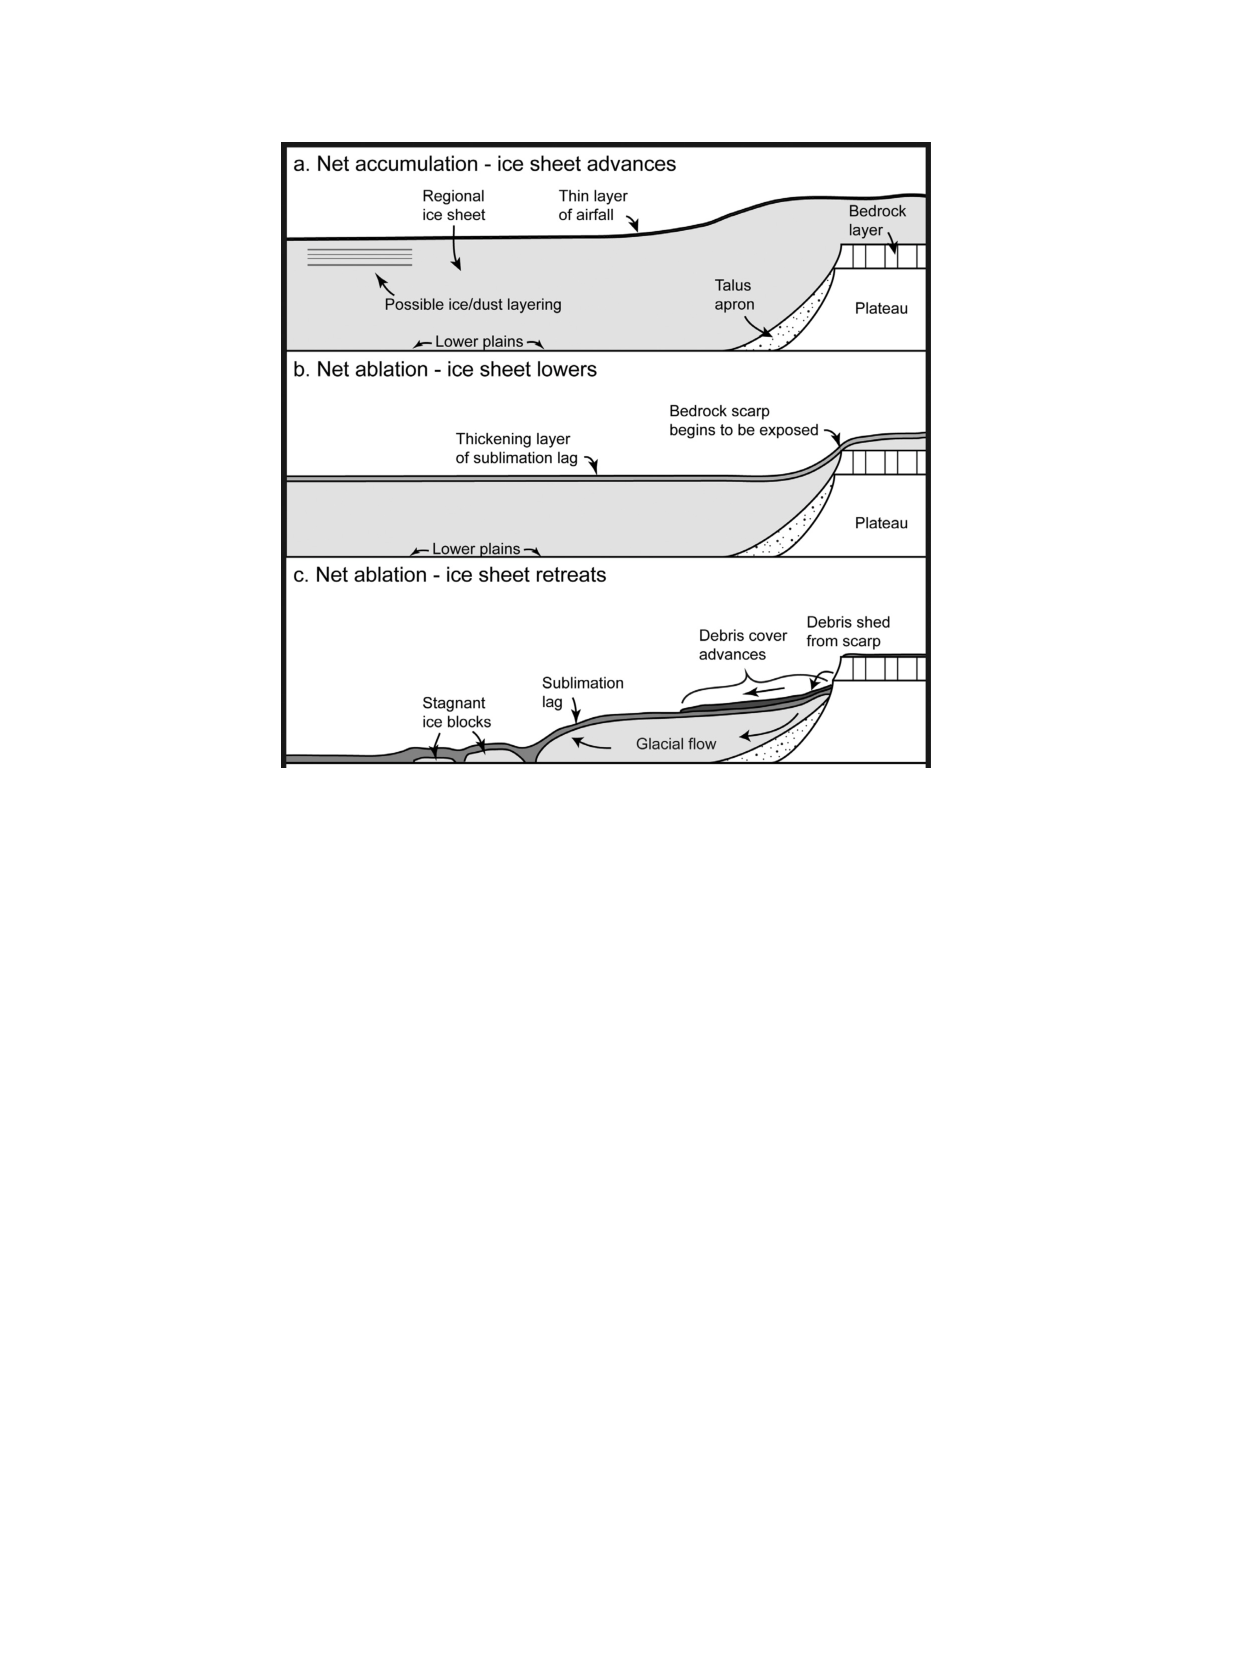
\includegraphics[
        width=\linewidth,
        height=0.65\textheight,
        keepaspectratio
    ]{Figures/Diagrams/Baker15_Fig17a.pdf}
\end{subfigure}
\hfill
\begin{subfigure}{0.48\textwidth}
    \centering
    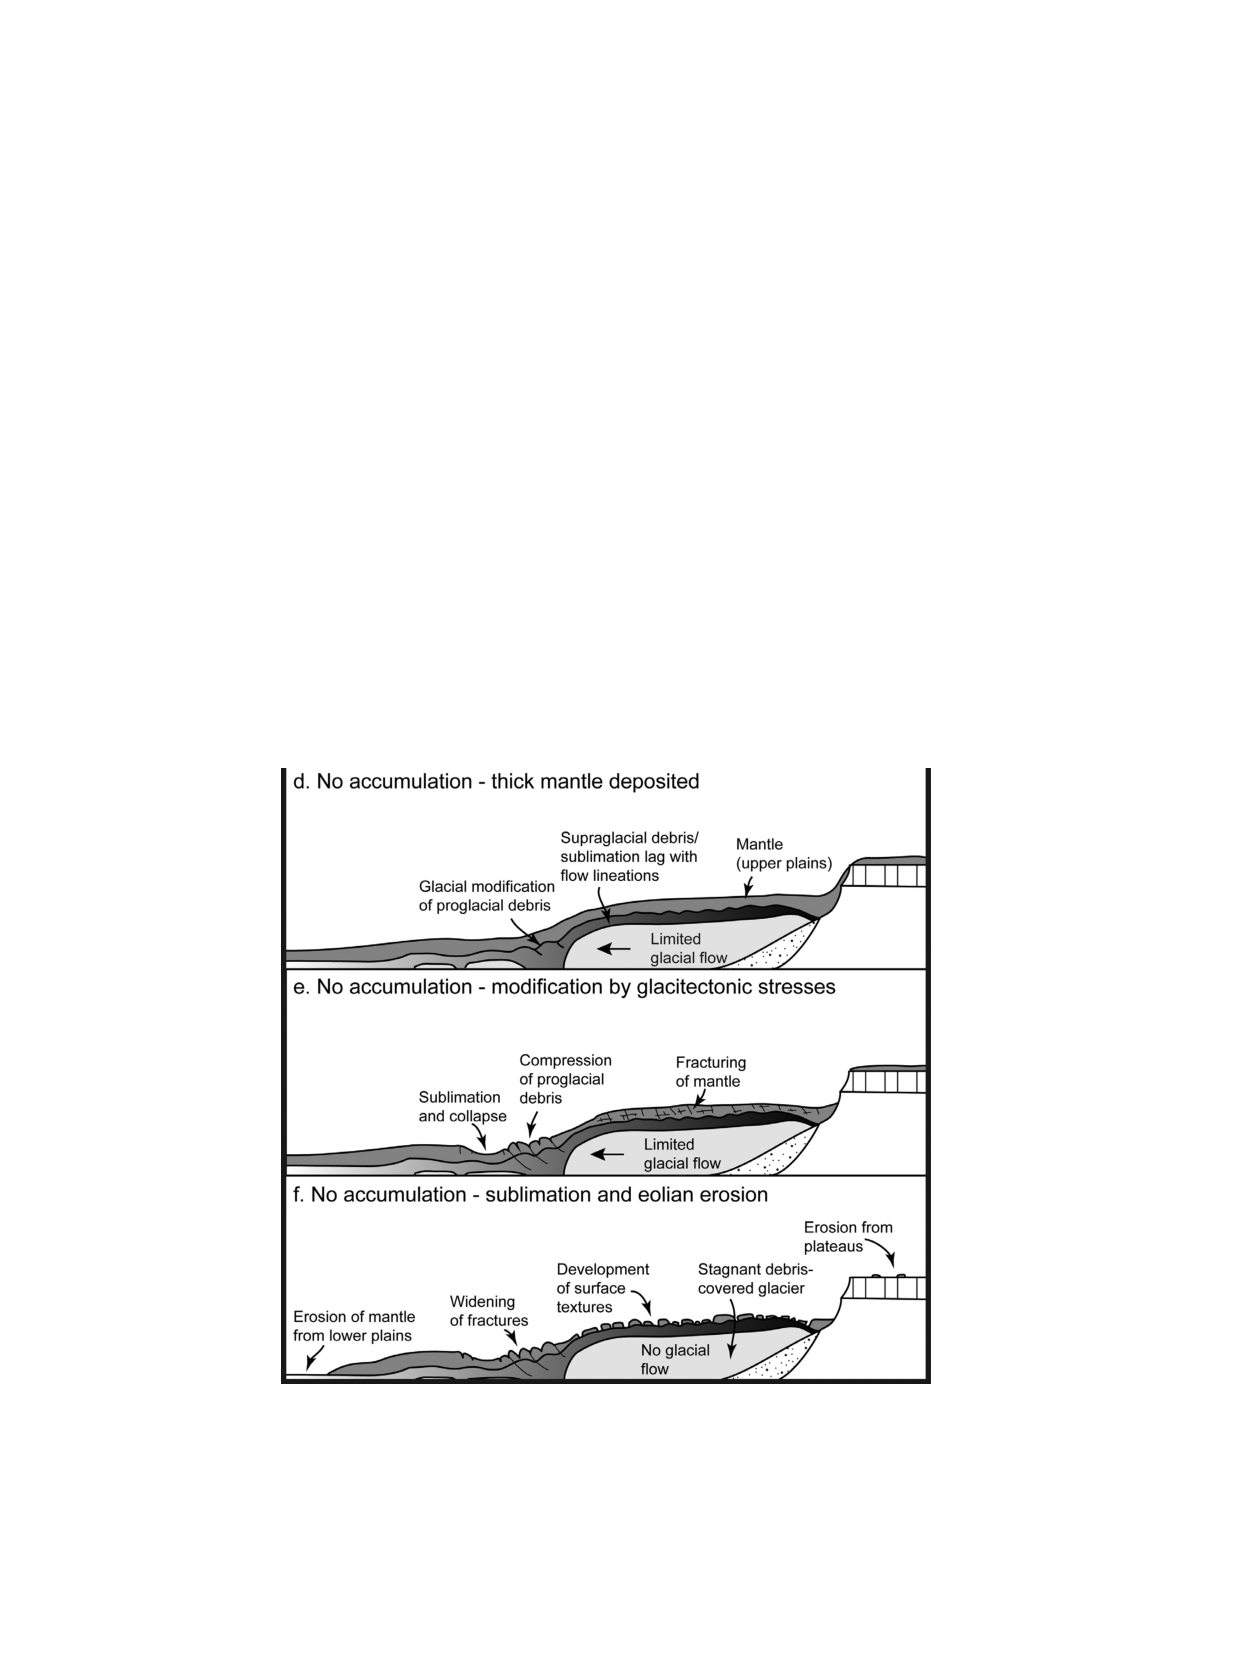
\includegraphics[
        width=\linewidth,
        height=0.65\textheight,
        keepaspectratio
    ]{Figures/Diagrams/Baker15_Fig17b.pdf}
\end{subfigure}
\caption{Schematic showing the mechanism of formation for glacier-related surface features (Figure from \cite{Baker15}).}
\label{fig:Baker15}

\end{figure}
\end{frame}
%%%%%%%%%%%%%%%%%%
\begin{frame}[label=RingMold]{Small-Scale Features: Craters}
\begin{figure}
    \centering
    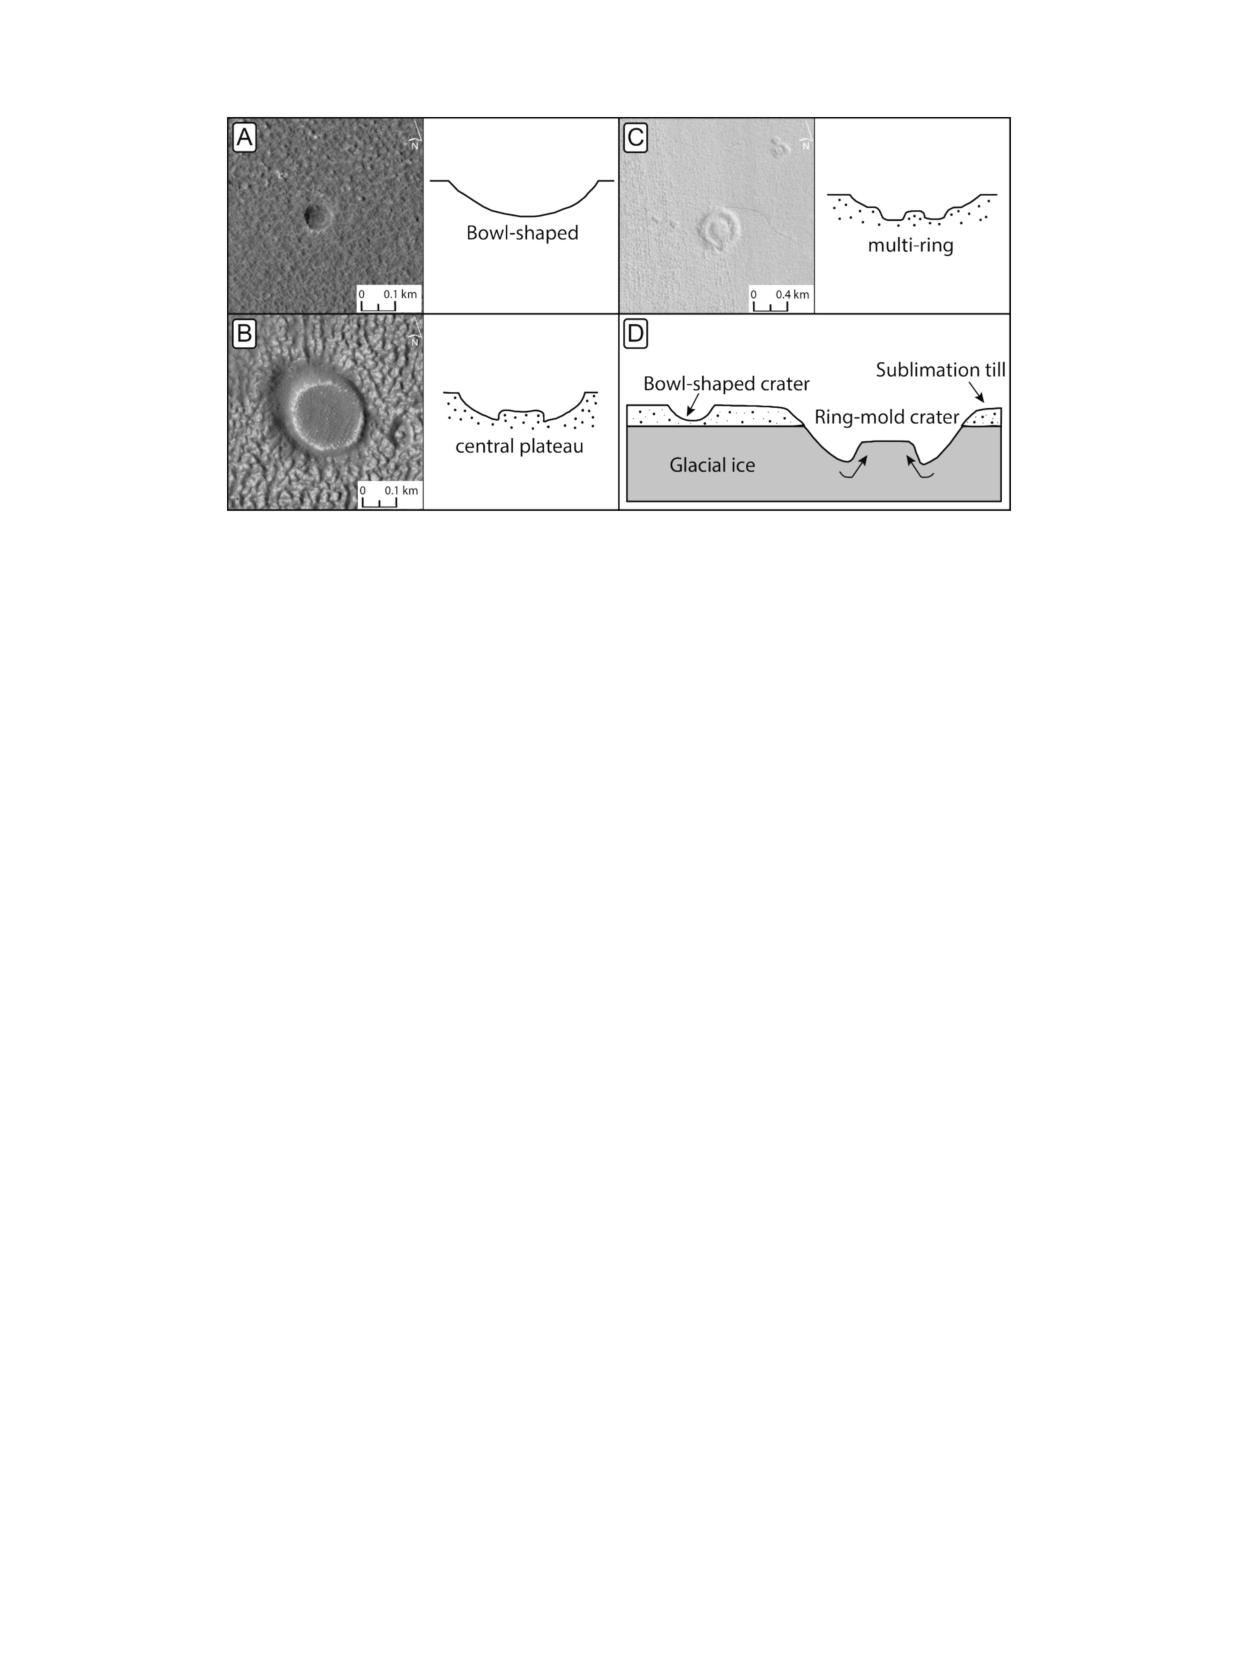
\includegraphics[
        width=\linewidth,
        height=0.65\textheight,
        keepaspectratio
    ]{Figures/Diagrams/Wueller25_Fig6.pdf}
    \caption{Diagram comparing the formation of bowl-shaped and ring-mold craters (Figure from \cite{Wueller25}).}
\label{fig:Wueller25_Fig6}
\end{figure}
\end{frame}
%%%%%%%%%%%%%%%%%%
\begin{frame}[label=SmallVFFs]{Small-Scale Features}
\begin{figure}
    \centering
    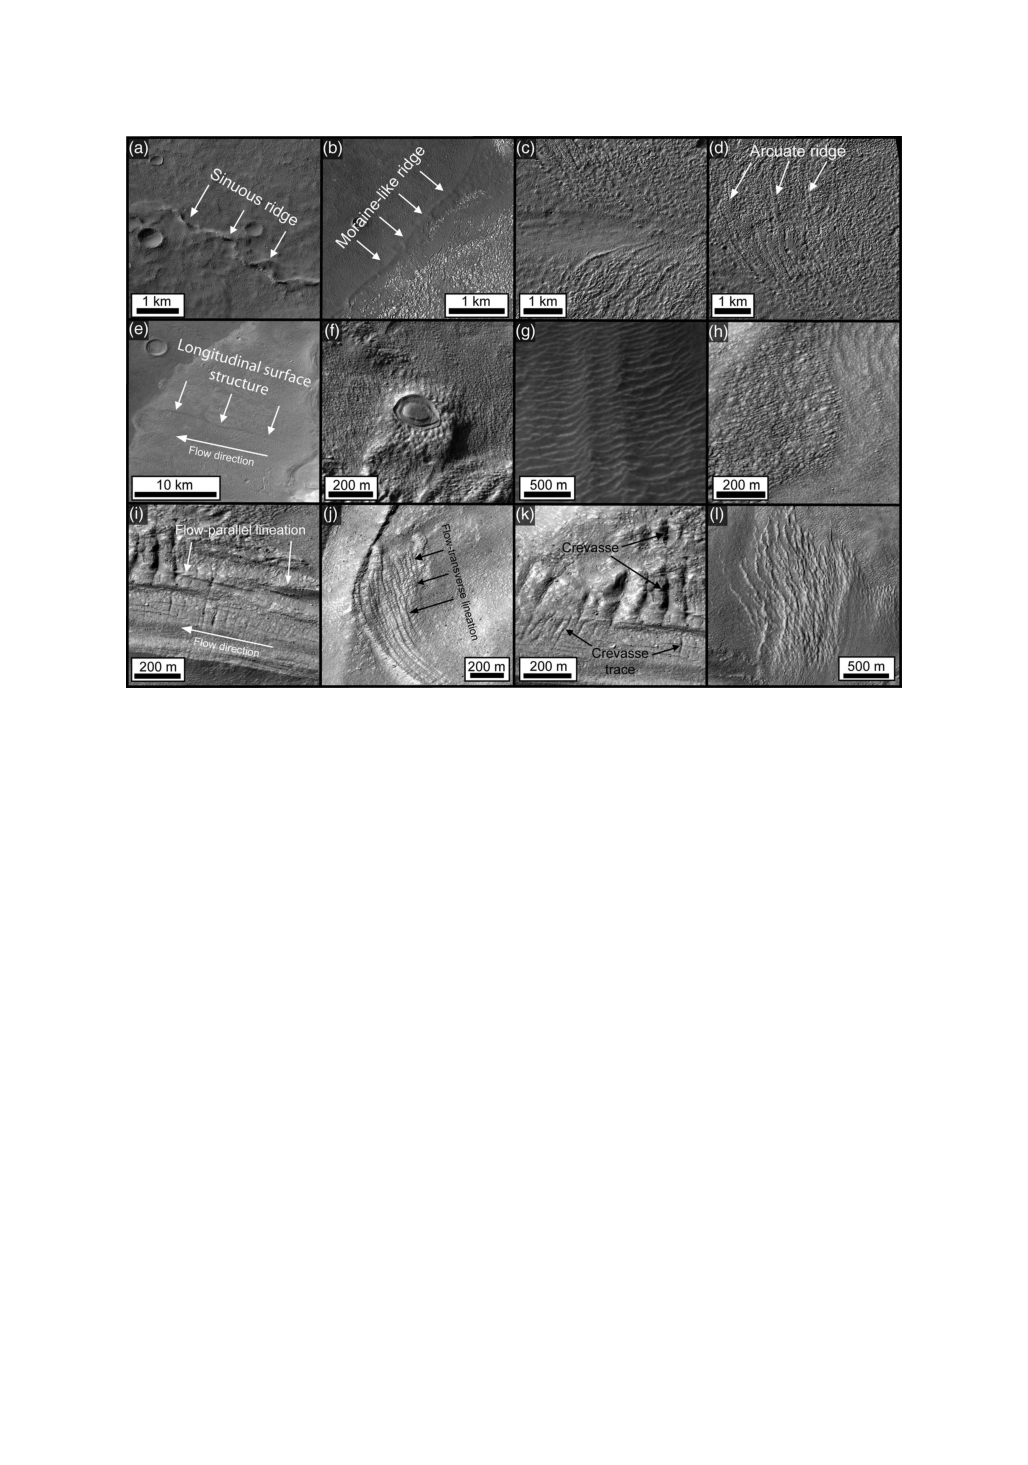
\includegraphics[
        width=\linewidth,
        height=0.65\textheight,
        keepaspectratio
    ]{Figures/Diagrams/Brough16_Fig3.pdf}
    \caption{Comparison between different surface features resulting from sublimation (Figure from \cite{Brough16}).}
    \label{fig:ButcherMangold_a}
\end{figure}
\end{frame}